\documentclass[hyperref={pdfpagelabels=false}]{beamer}
\usepackage[BoldFont,SlantFont,CJKnumber,CJKchecksingle]{xeCJK}  
\usepackage{lmodern}
\usetheme{CambridgeUS}
%%%%%%%%%%%%%%%%%%%%%%%%%题目,作�
\title{Plankton Classification of WHOI}  
\author{Jinna Cui} 
\institute{Vision Lab of OUC}
\date{2016.11.28} 
\begin{document}
\logo{
\includegraphics[scale=0.3]{visionouc.jpg}}
\begin{frame}
\titlepage
\end{frame} 


\begin{frame}
\frametitle{Table of contents}
\tableofcontents
\end{frame} 


\section{Introduction of WHOI} 
\begin{frame}
\frametitle{Introduction of WHOI} 
\begin{itemize}

\textbf{\Large{WHOI}}
 \newline
  \newline
   \newline
   \newline
\item \textbf{Large:} 103 classes & more than 3.56 millions images
 \newline
 \newline
 \newline
\item \textbf{Imbalance:} 5 large classes
 \newline
 \newline
 
\end{itemize} 
\end{frame}



\begin{frame}
\frametitle{Filter}
\centering

\begin{figure}[!htb] %插
\centering
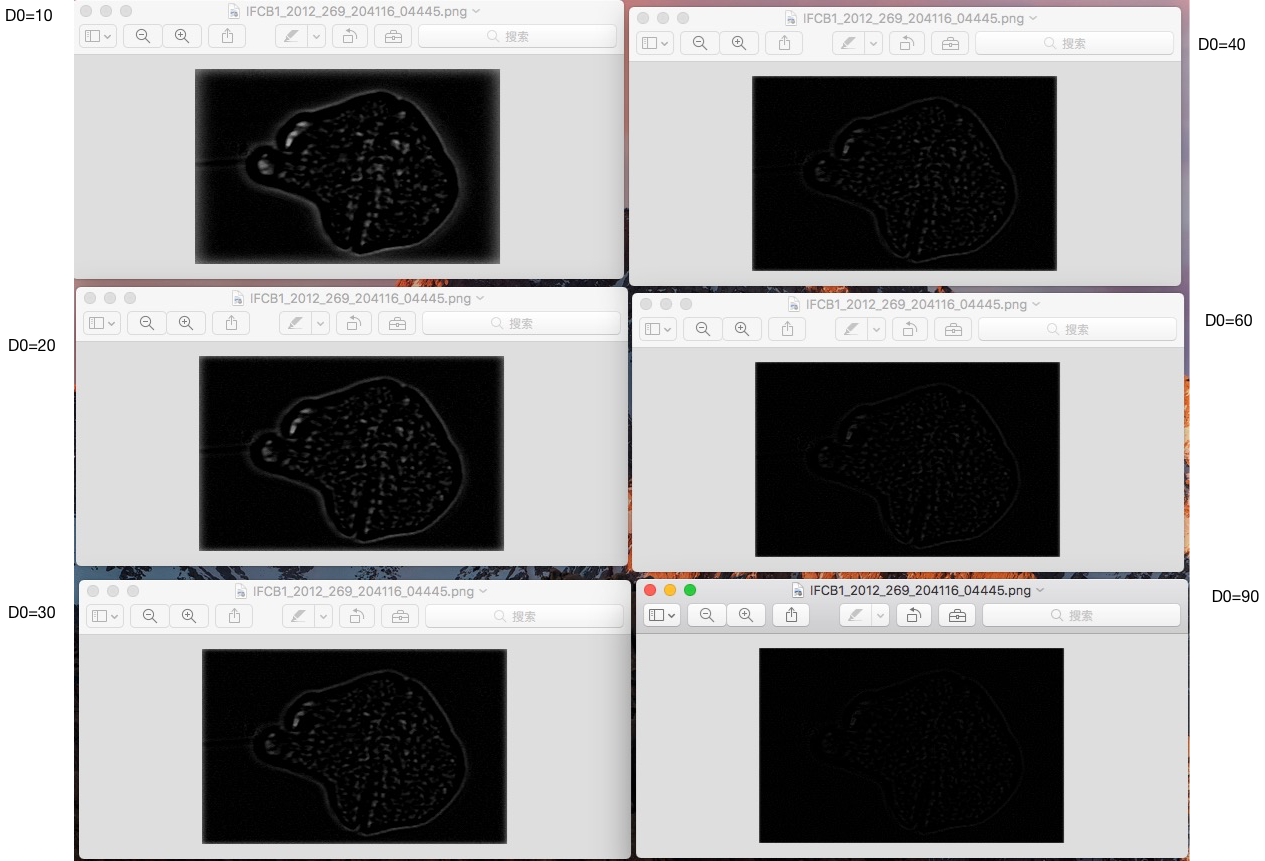
\includegraphics[width=0.45\textwidth]{gaotong}
\centering
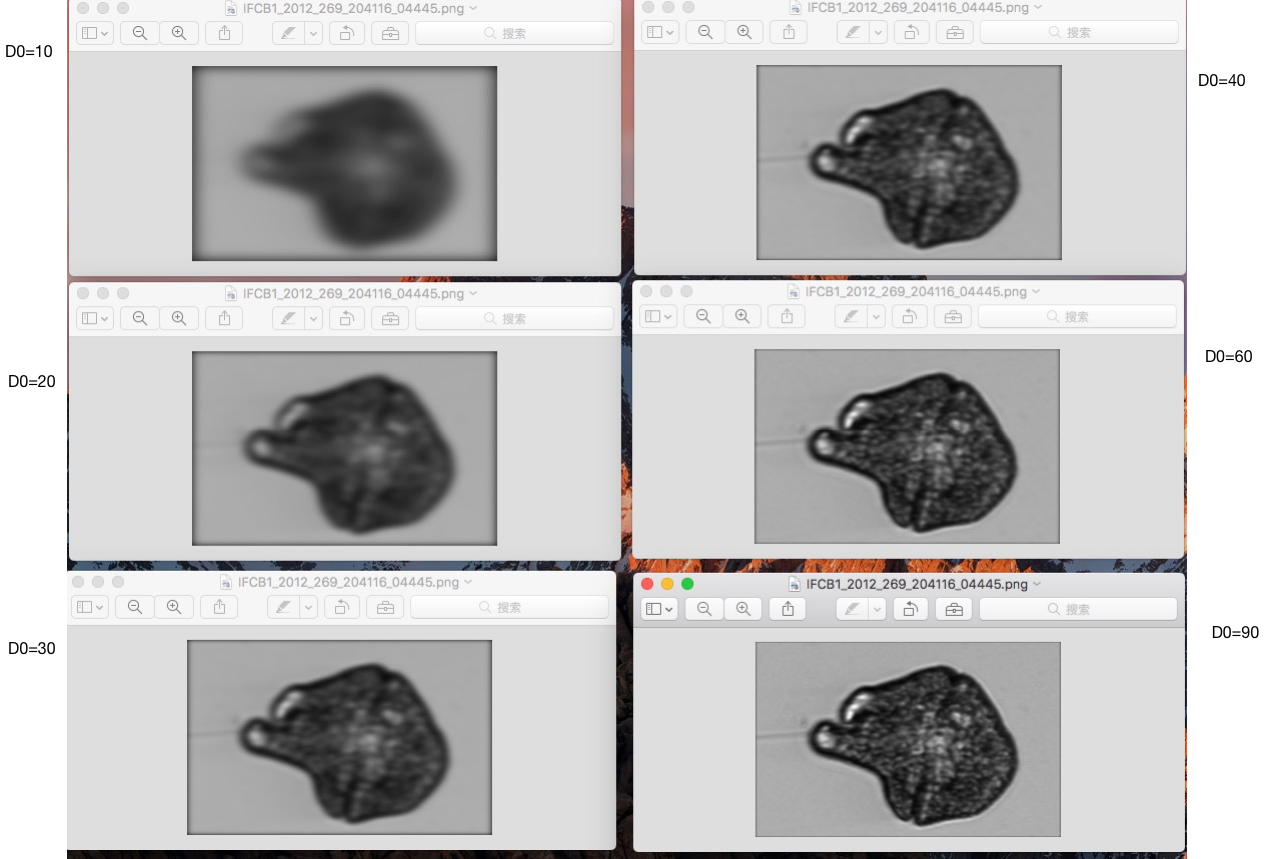
\includegraphics[width=0.45\textwidth]{ditong}
\end{figure} 
\end{frame}



\section{Introduction of Neural Network Architecture} 
\begin{frame}\frametitle{Architecture of Neural Network}
\centering

\begin{figure}[!htb] %插
\centering
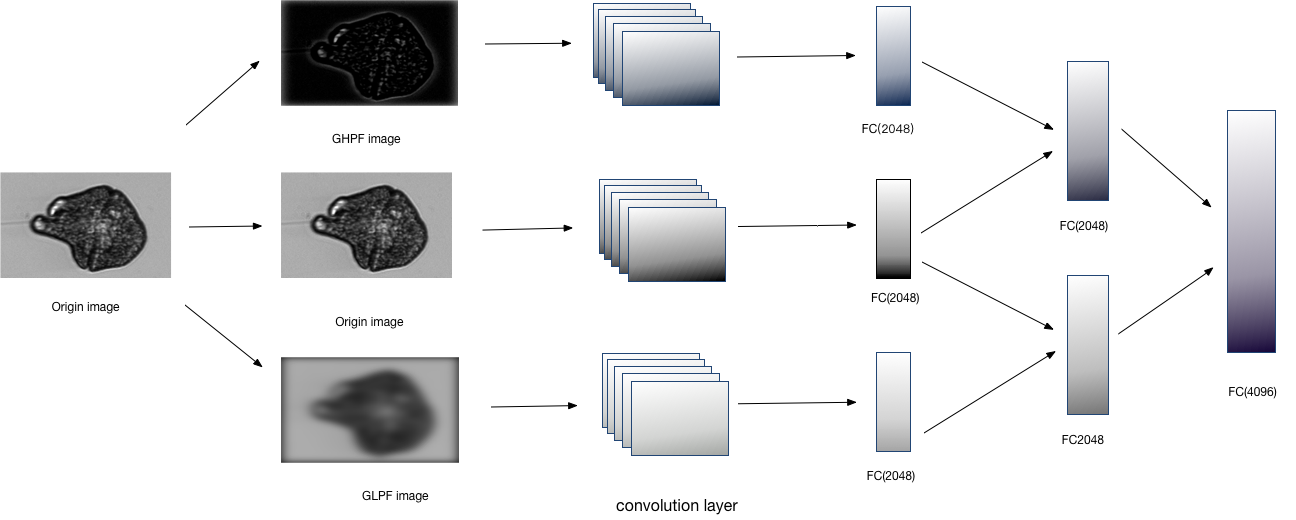
\includegraphics[width=0.8\textwidth]{network}
\end{figure} 
\begin{itemize}
\item Convolutional Neural Network
 \newline
\item 3 channels (share same label)
 \newline
\item Pyramid fully connected structure
\end{itemize} 
\end{frame}

\section{Results of My Experiments} 
\begin{frame}\frametitle{Experiments Results}
\centering

\begin{table}[tbp]
\centering  % ???
\begin{tabular}{lccc} 
\hline
Models \ \   &Accuracy\\ \hline  
AlexNet trained on origin images &93.58\% \\  \hline       
AlexNet trained on 3 channels images &94.21\%\\  \hline      
\end{tabular}
\caption{\scriptsize{Experiments Results of Plankton Classification}}
\end{table}

\end{frame}


\begin{frame}
\center
\huge{Thanks for your attention !}
\end{frame}


\begin{frame}
\center
\Huge{Q \& A}
\end{frame}
\end{document}
